\chapter{Introduction}\label{cha:intro}
Discrepancies in measurements of the rotations of galaxies indicate the presence of a large amount of matter which interacts through gravity, though not electromagnetically making it invisible to our telescopes. This matter is commonly referred to as dark matter. Since no known or hypothesised particle in the standard model of particle physics can be used as a candidate for dark matter, this has opened the door for new physics. Aside from dark matter there are other phenomena, such as the neutrino mass and the hierarchy problem, that can not be explained today.  

At the Organisation européene pour la recherche nucléaire (\abbrCERN) the interest now lies to discover any evidence of so called weakly interacting massive particles (\abbrWIMPS) which may be a candidate for dark matter. It is usually impossible to detect any interaction of dark matter candidates on the subatomic scale, however through looking at proposed interactions, searching for assumed decay channels and inconsistencies in momentum conservation it is hoped that signs will be found. Though as of \today , none have been found. 

Both these experiments and current theories now show that higher energies are required at the \abbrLHC to be able to see any signs. This is why the \abbrLHC and all detectors are undergoing a vast upgrading program \citep{ATLAS:LOI2}.
In this thesis focus will be on the last part of the upgrade due for completion in 2023, known as the high luminosity-\abbrLHC phase II upgrade; and also on the \abbrATLAS detector. The method used in this thesis focuses on looking as data which emulate conditions at the upgraded \abbrLHC.

\newpage
\section{Research goals}\label{sec:goals}
This research took place at Stockholm University from January 7th until \textbf{when?}
During the research period the following tasks were set up and performed/answered:
\begin{itemize}
\item Implement a C++ programme that loops over the collisions inside the signal and background datasets.	
\item For each collision retrieve the relevant observables (variables used to	 extract the signal over the background) and apply "smearing functions" to emulate the effect of the high luminosity on the observables. 	
\item For both signal and background datasets, compare observables before and after smearing. What observables are the least/most affected?	
\item Implement selection criteria that selects the signal collisions efficiently while reduces significantly the background. In a first step the selection criteria should be taken from existing studies.
\item Selection criteria can be evaluated and compared with each other using a figure of merit P, that measures the sensitivity of the experiment to the	 dark matter signal. Calculate P for the given selection criteria before and after smearing.
\item What is the effect of the high luminosity (smearing) on the value of P?
\item Investigate other selection criteria and observables, to mitigate the effect of high luminosity. Use P to rank different criteria after smearing.
\item Conclude on the effect of the high luminosity on the sensitivity for dark matter and possible ways to mitigate its effects using alternative observables and selection criteria. 
\end{itemize}
\newpage
\section{Theoretical Background}\label{sec:tb}
The following is a short description of the theory which is required to understand this thesis. 
\subsection{Quantum mechanics and quantum field theory}\label{sec:tb:subsec:qm}
In the beginning of the 20th century, some physical phenomena could not be explained by classical physics, for example the ultra-violet disaster of any classical model of of black-body radiation, and the photoelectric effect \citep{Bransden:2000}.
It was these phenomena that led to the formulation of quantum mechanics (\abbrQM), where energy transfer is quantized and particles can act as both waves and particles at the same time \citep{Hallsjo:2013}.

Combining \abbrQM with classical electromagnetism proved harder than expected, colliding a photon(em-field) and an electron (particle/wave) is quite tricky. This can be seen when trying to calculate the scattering between them both in a \abbrQM schema. One idea that came from this was to explain them both in the same framework, field theory. Also, trying to incorporate special relativity into \abbrQM suggested a field description where space-time is described using the metric formalism from differential geometry.
The culmination of both of these problems is the first part of a Quantum field theory (\abbrQFT), Quantum electrodynamics (\abbrQED) which with incredible precision explains electromagnetic phenomena including effects from special relativity\citep{Zee:2003}. It is in this merging that antimatter was theorised, since it is a requirement for the theory to hold. After the discovery of antimatter, the theory was set in stone. Since this the theory has been altered somewhat to explain more and more experimental data. This is discussed more in \subsectionref{sec:tb:subsec:nps} and \subsectionref{sec:tb:subsec:SM}.

To be able to calculate properties in \abbrQFT one uses the Lagrangian formalism \citep{Goldstein:2001}. Which gives a governing equation for the different physical processes. In general the Lagrangian used for the Standard model is quite complicated, one can thus focus on one of the different terms corresponding to a specific force. This can be done to calculate the so called cross-section for a process, which is related to the probability that that process will occur. A step to simplify the calculations is to use the so called Feynman diagrams, an example of which is given in \figureref{fig:exFeynman}. 

\begin{SCfigure}[][h]
 \centering
 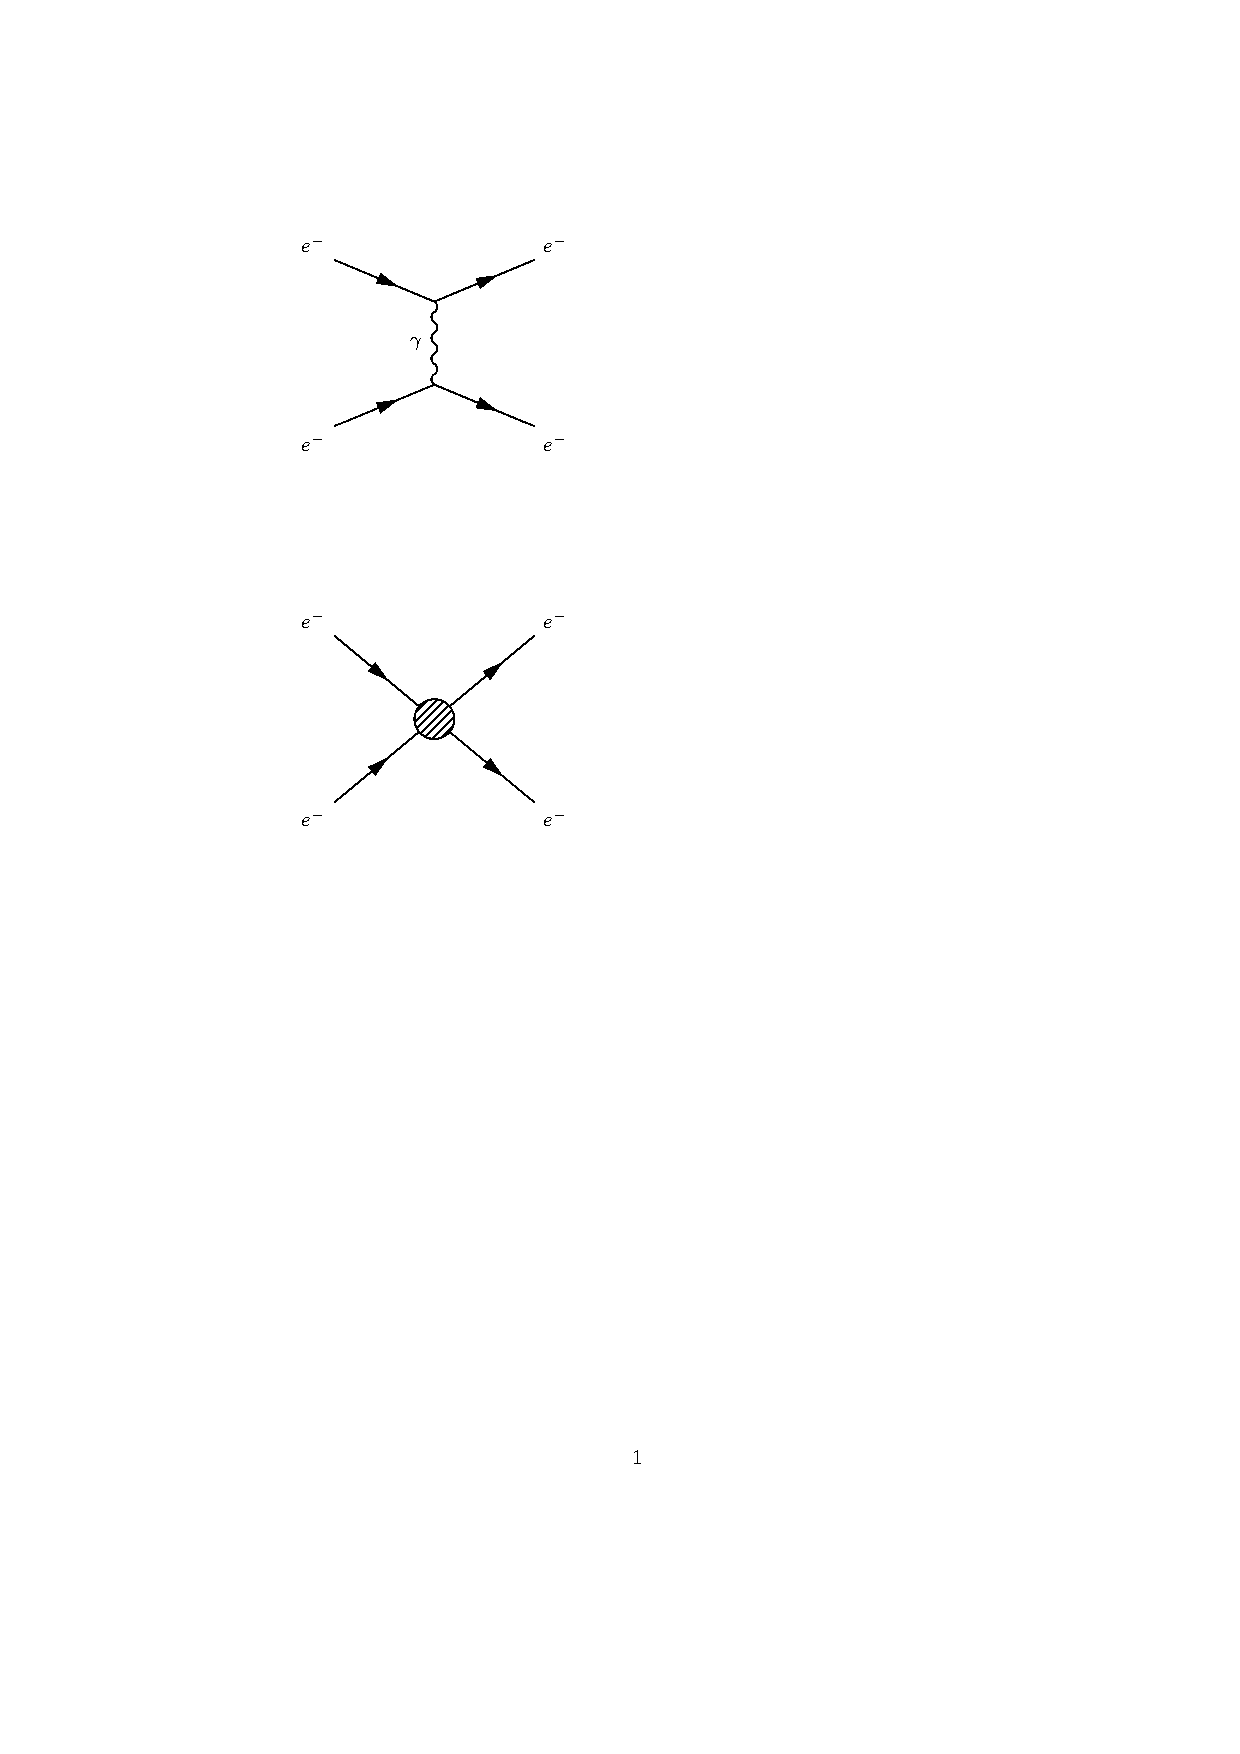
\includegraphics[trim=5cm 22cm 11cm 4cm,clip=true, width=0.4\textwidth]{myfeynman.pdf}
  \caption{{\small An example of a Feynman diagram explaining an electron-electron scattering using \abbrQED.}}
    \label{fig:exFeynman}
\end{SCfigure}

Through the figure, which comes with certain rules, and knowing what the major process (in this case \abbrQED) one can calculate the cross-section \citep{Zee:2003}. it is this that is needed to predict is one will be able to detect new particles. 

\subsection{Nuclear, particle and subatomic particle physics}\label{sec:tb:subsec:nps}
Many could argue that these branches of physics started after Ernest Rutherford famous gold foil experiment \citep{Burchan:1995}, where he discovered that matter is composed of matter with a nucleus, a lot of empty space and electrons. 

It was this and other things that sparked the curiosity to see what the nucleus is made of and what forces govern the insides of atoms. After this, and the combination of the theoretical description given by \abbrQM, a lot more has been discovered and still more has been predicted. The newest of these is of course the Higgs particle, which was predicted through \abbrQFT and then discovered by \abbrCERN \citep{Higgs:2012}. 

The discovered particles are often divided into different groups depending on the fundamental particles that build them up. For instance, particles build up of three quarks are known as hadrons. Particles with an integer spin are known as bosons whereas half-integer particles are known as fermions.

\subsection{The standard model of particle physics}\label{sec:tb:subsec:SM}
The standard model of particle physics, referred to simply as the standard model (\abbrSM), is the particle zoo which tries to categorize all the particles and that have been discovered experimentally. \abbrQFT has tried its best to explain the interactions between these particles and it has also predicted several particles by including symmetries \citep{Burchan:1995}. Regarding \abbrSM, Gauge bosons are the force carriers for the different forces, quarks are the and leptons are the fundamental blocks that we know of so far. The difference between the later two is if they interact via the strong force or not. 
\begin{SCfigure}[][h]
 \centering
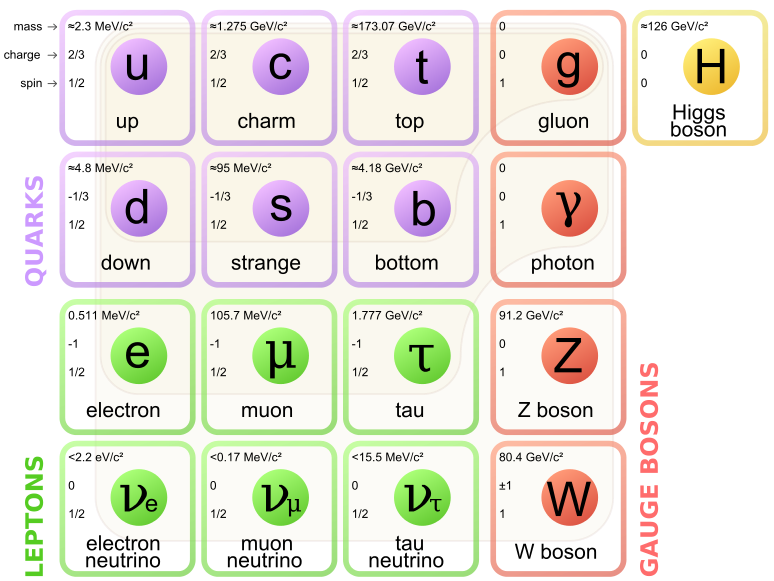
\includegraphics[scale=0.2]{Standard_Model_of_Elementary_Particles.png}
  \caption{{\small The standard model of particle physics where the three first columns represent the so called generations, starting with the first. \citep{wiki1}.}}
    \label{fig:SM}
\end{SCfigure}

\abbrSM is today the pinnacle of particle physics and can be used to explain almost everything that occurs around us. There are however some problems \citep{Jungman:1996}:
\begin{itemize}
\item No \abbrQFT for general relativity! Thus there is no link between gravity and the \abbrSM.
\item Experimentally it has been shown that neutrinos have mass, though in \abbrSM they do not!
\item Asymmetry between matter and antimatter can not fully be described.
\item No dark matter candidate!
\item No explanation that can contain dark matter.
\end{itemize} 
In this thesis focus lies with dark matter, some more introduction to possible dark matter and different candidates in extensions to \abbrSM are explained in \subsectionref{sec:tb:subsec:dark}.


\subsection{Dark matter}\label{sec:tb:subsec:dark}
A very quick introduction was given in the beginning of this chapter. Dark matter is the name given to the solution to the discrepancies of galactic rotations. 


To explain this, focus on matter in a galaxy which are rotating around the center of the galaxy. Through Newtons law of gravity and the centrifugal force one can calculate the rotation speed dependent on the distance to the center of the galaxy. Since one of these forces is attractive and the other repulsive, if the matter is in a stable orbit around the galactic center (which they are) they must be equal and give us an expression for the speed depending on the distance. Newtons law can be written as the following:
\begin{equation}\label{eq:forces}
F_{Gravitational}=G \frac{M m}{r^2} = G_M \frac{m}{r^2} \qquad F_{Centrifugal} = m\frac{V^2}{r}
\end{equation}
where G is the gravitational constant, M the mass of the centre object, m the mass of the matter, r the distance between the two and V is the rotation speed. It has been simplified using $G_M$ since all matter orbits the same galactic center. Setting the equations in \eqref{eq:forces} results in:
\begin{equation}\label{eq:rotation}
G_M \frac{m}{r^2} = m\frac{V^2}{r} \Leftrightarrow V^2 =\frac{G_M}{r} \Rightarrow V=\sqrt{\frac{G_M}{r}} \propto \frac{1}{\sqrt{r}}
\end{equation}
where the speed is assumed to be positive and $\propto$ means proportional. Through these simple calculations it shown that the rotation speed should decrease with and increased distance. The same reasoning can be applied to, our solar system where this is the case \figureref{fig:rotation:a}. The relation in these units is $V=\frac{107}{\sqrt{r}}$ where 107 can be used in \eqref{eq:rotation} to calculate the mass of the sun. However when looking at galaxies, even when taking into account that one has to see the galaxies as a mass distribution and that the above is only true when outside of the inner mass half, this is not the case! In \figureref{fig:rotation:b} experimental data can be seen from the galaxy NGC3198 with a fitted curve which does not decrease with the distance but is instead constant.  This is the discrepancy which is solved by postulating the existence of dark matter.
 \begin{figure}[h] %!ht
    \subfloat[Rotation speed of planets in our solarsystem. Based on data from \citep{Nasa}. \label{fig:rotation:a}]{%
     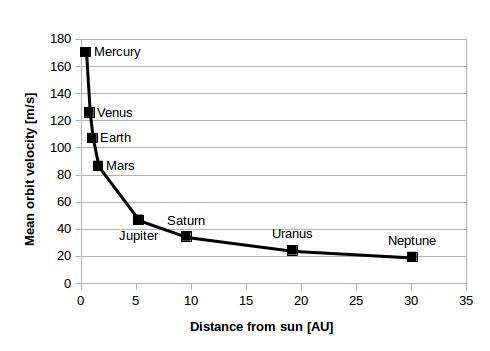
\includegraphics[width=0.5\textwidth]{solarsystemrotation2.jpg}
    }
    \hfill
    \subfloat[Rotation speed of mater in NGC3198 with a curve fitting and three different models, if only a dark model halo existed, if there was no dark matter and the correct, if both exist \citep{Albada:1985}.\label{fig:rotation:b}]{%
      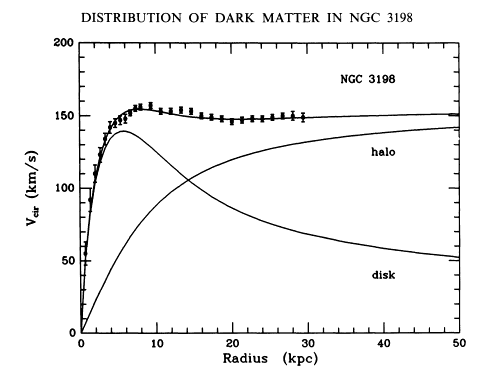
\includegraphics[width=0.5\textwidth]{rotationNGC3198.png}
    }
    \caption{Different rotation curves, both for planets in our solar system and matter in the NGC3198 galaxy.}
    \label{fig:rotation}
  \end{figure}
After this the big question arises, what could this dark matter consist of? What is known so far lies in the name. Dark since no electromagnetic interaction and matter since gravitational interaction. This means that it can not be made up of any barionic matter or anything in the Standard Model apart from neutrinos. The main topic and also the main contributor to the rotational discrepancies is known as cold dark matter. This is due to the matter having as low kinetic energy and have mass in the GeV scale \citep{Goodman:2010,CERN-PH-EP-2012-210,Jungman:1996}. This means however that neutrions can not be a candidate, thus the standard model is ruled out. 
There are several different ideas for how dark matter can be detected, \citep{Jungman:1996}
\begin{itemize}
\item Ordinary matter interacting with ordinary matter can produce dark matter, known as production.
\item Dark matter interacting with ordinary matter can produce dark matter, known as direct detection.
\item Dark matter interacting with dark matter can produce ordinary matter, known as indirect detection.
\end{itemize} 
In this theses the focus lies with production. There are several theories how to detect dark matter in proton-proton collisions such that occur at \abbrCERN this is covered more in \subsectionref{sec:tb:subsec:WIMPS}. 

\subsection{Effective field theory}\label{sec:tb:subsec:eft}
In quantum field theory the objective is usually to find the part of the Lagrangian which explains a type of interaction, known as the operator of the interaction and also to find the probability amplitude (cross-section) for a certain interaction. For complicated processes it is easier to employ certain conditions so that the small scale phenomena are simplified and the whole picture understood. This called using an effective field theory and the idea can be in \figureref{fig:feymanc}. The operator can be found through assuming the possible interactions and using the effective field theory \citep{Zee:2003}. The cross-sections can be found through the Feynman diagrams as described in \subsectionref{sec:tb:subsec:qm}. 
%trim=left botm right top.
 % good for finding limits \fbox{\includegraphics}
 \begin{figure}[H] %!ht
    \subfloat[Electromagnetic interaction.\label{fig:feymanc:a}]{%
     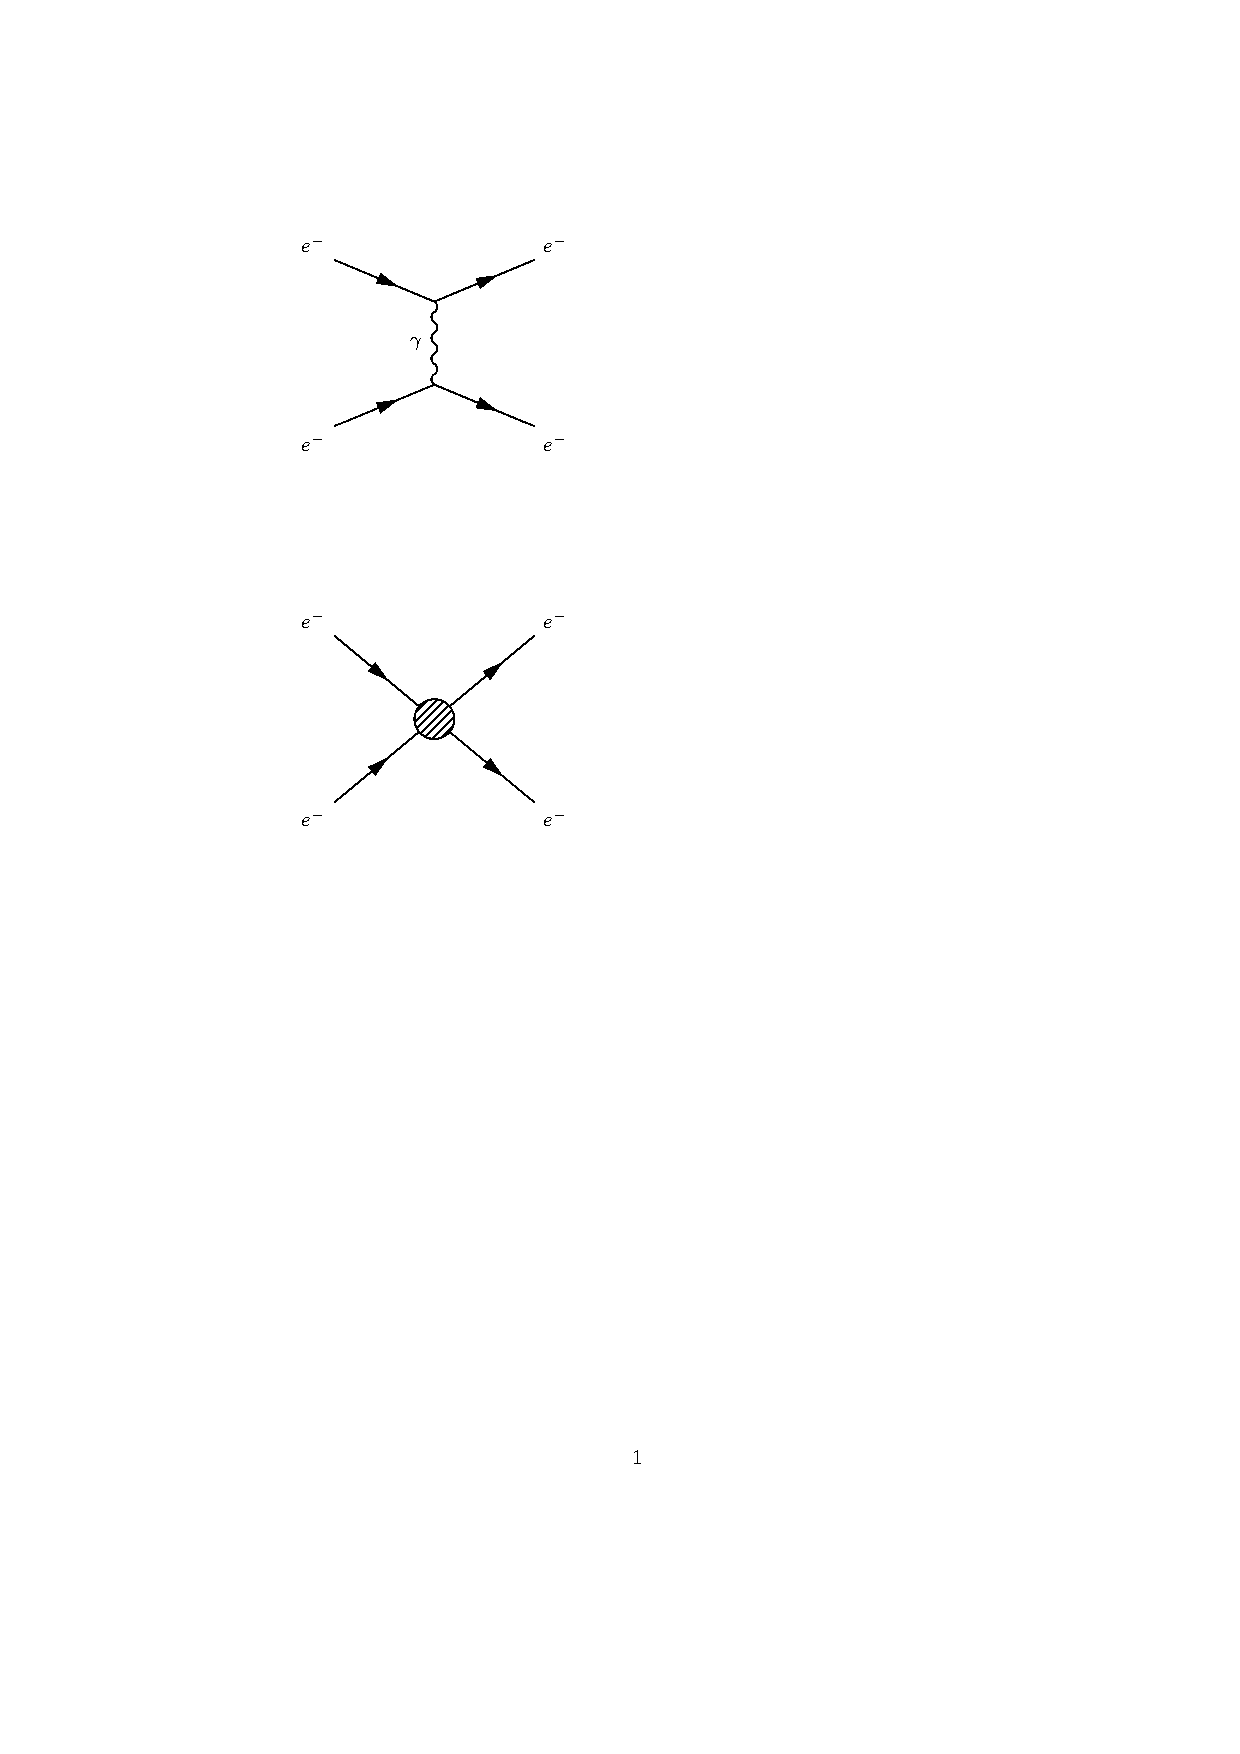
\includegraphics[trim=5cm 22cm 11cm 4cm,clip=true, width=0.5\textwidth]{myfeynman.pdf}
    }
    \hfill
    \subfloat[Effective diagram of \figureref{fig:feymanc:a}.\label{fig:feymanc:b}]{%
      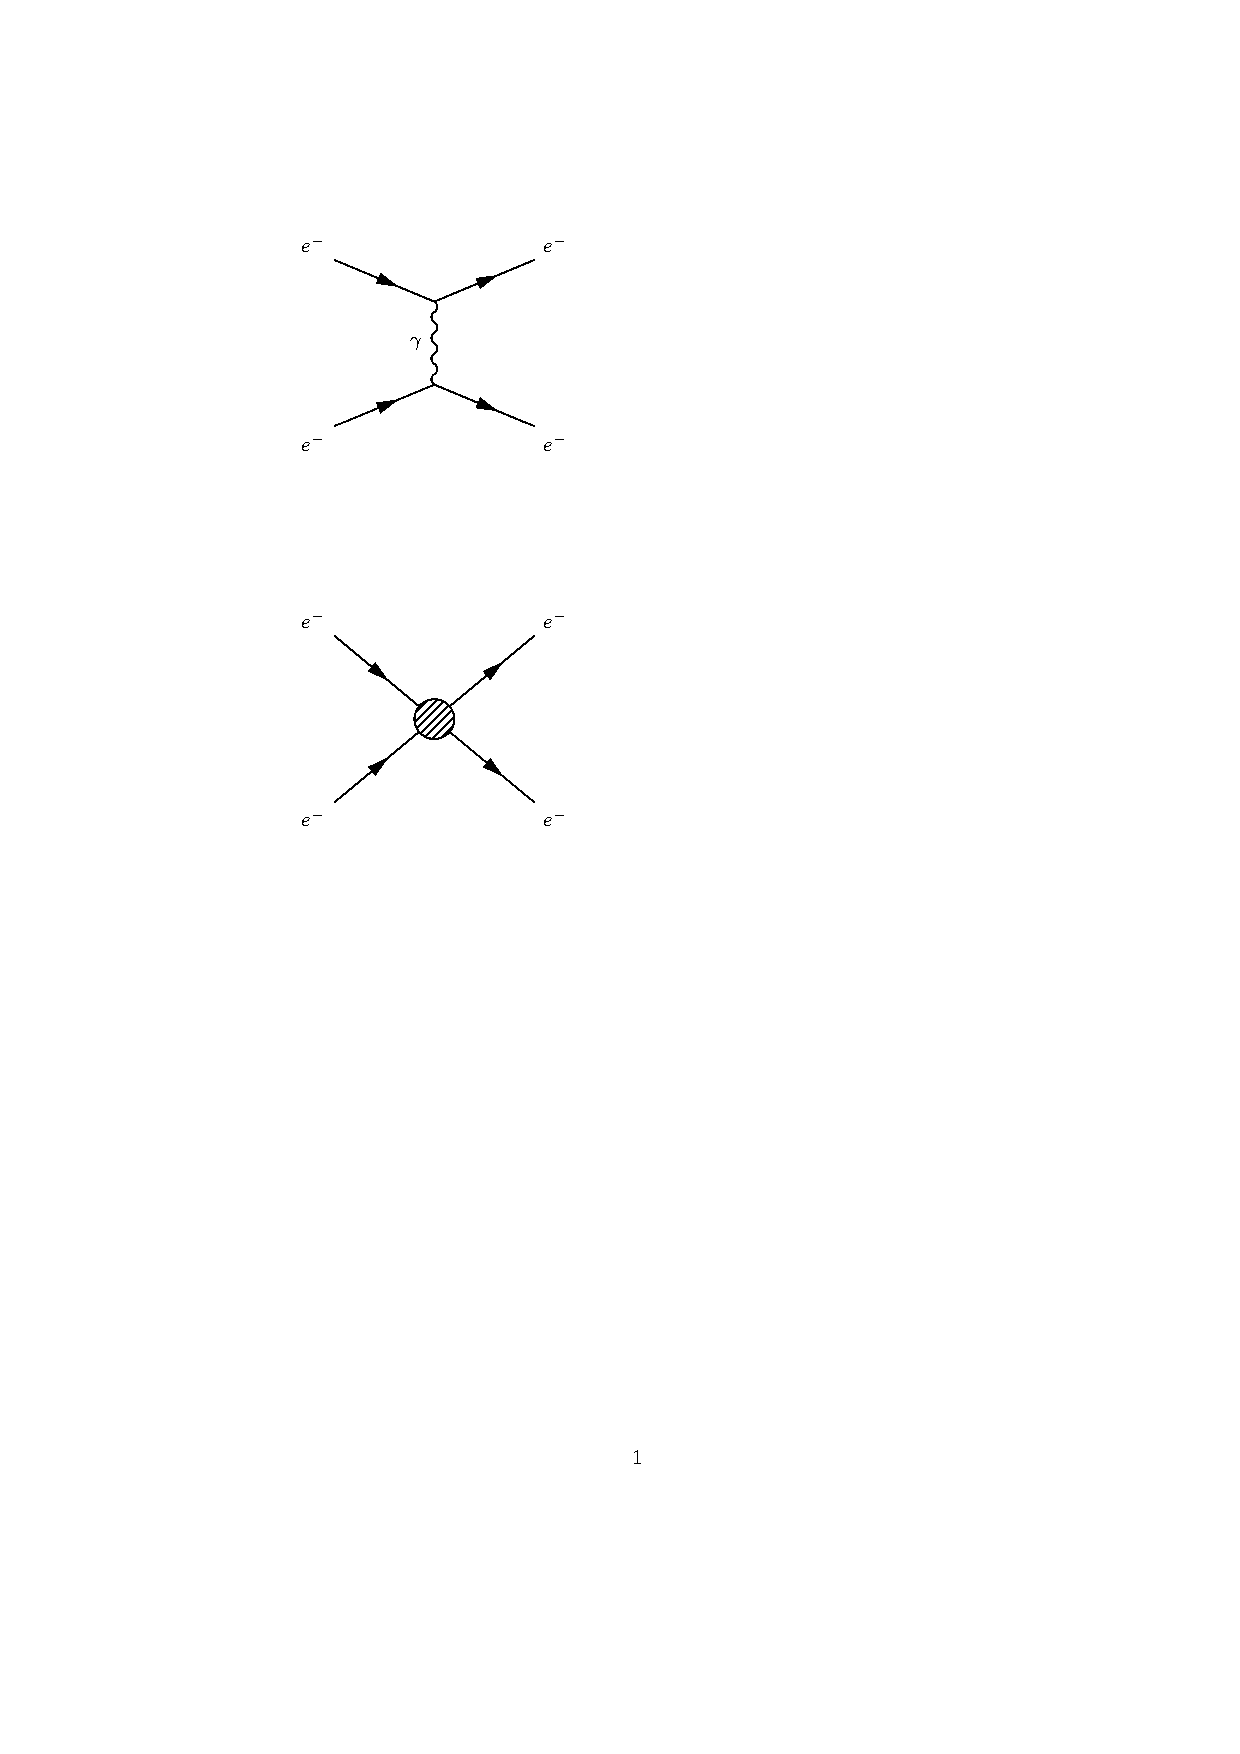
\includegraphics[trim=5cm 15.7cm 11cm 10.3cm,clip=true, width=0.5\textwidth]{myfeynman.pdf}
    }
    \caption{Feyman diagram of an electron-electron scattering, both as an ordinary diagram and as its effective version, where the details are hidden in the blob.}
    \label{fig:feymanc}
  \end{figure}
In this thesis the same effective field theory as in \citep{82.116010,Goodman:2010} will be considered. The \abbrWIMP (usually denoted $\chi$) is assumed as the only particle in addition to the standard model fields. $\chi$ will be assumed odd under some $Z_2$ symmetry. This means that an even number of $\chi$ must be in every coupling. It is assumed that the whatever mediator exists is heavier that the \abbrWIMPS, meaning that their interactions are in higher order terms of the effective field theory and thus not included in the operators. For simplicity, the \abbrWIMPS are assumed to be \abbrSM singlets, thus invariant under \abbrSM gauge transformations, and the coupling to the Higgs boson is neglected.

The focus for the operators will be quark bilinear operators on the form $\bar{q}\Gamma q$ where $\Gamma$ is a 4 $\times$ 4 matrix of the complete set, 
\begin{equation}
\Gamma = \left\lbrace 1,\gamma ^5,\gamma ^\mu,\gamma ^\mu \gamma ^5, \sigma ^{\mu \nu} \right\rbrace
\end{equation}
This will dictate how the operators are written, more of why this is done can be found in \citep{82.116010,Goodman:2010,Zee:2003}.

This, together with the coupling with the strong force defines an effective field theory of the interaction of singlet \abbrWIMPS with hadronic matter. It is a non-renormalizable field theory which will break down when the mediator mass is close to the mass of the \abbrWIMP .
The condition for this is derived in \citep{82.116010} and gives:
\begin{equation}
M > 2 m_\chi
\end{equation}
where $m_\chi$ is the mass of the \abbrWIMP and M is the mass of the mediator. There is also the requirement that:
\begin{equation}
M \lesssim 4 \pi M_*
\end{equation}
where $M_*$ is the energy scale where the effective theory is no longer a good approximation.

In this work, WIMPS are assumed to be Dirac fermions (half integer spin and is not its own antiparticle). 
 
In \tableref{tab:operators} the operators which are integrated out via the effective field theory and are of interest in this thesis are given.
\renewcommand{\arraystretch}{1.5} %Change height of tabel
\begin{table}[H]
\begin{center}
    \begin{tabular}{ | l | l | l | l |}
    \hline
    Name & Initial state & Type & Operator \\ \hline
  	D1 & qq & scalar & $\frac{m_q}{M^3_*} \bar{\chi} \chi \bar{q} q$ \\ \hline
  	D5 & qq & vector & $\frac{1}{M^2_*} \bar{\chi} \gamma^\mu \chi \bar{q} \gamma_\mu q$ \\ \hline
  	D8 & qq & axial-vector & $\frac{1}{M^2_*}\bar{\chi}\gamma^\mu \gamma^5 \chi \bar{q} \gamma_\mu \gamma^5 q $ \\ \hline
  	D9 & qq & tensor & $\frac{1}{M^2_*} \bar{\chi}\sigma^{\mu \nu} \chi \bar{q} \sigma_{\mu \nu} q  $\\ \hline
  	D11 & gg & scalar & $\frac{1}{4M^3_*}\bar{\chi}\chi \alpha_s (G^a_{\mu \nu})^2 $\\ \hline
  	\end{tabular}

  	\caption{Table based on discussion in \citep{CERN-PH-EP-2012-210}}
  	\label{tab:operators}
  	  	\end{center}
    \end{table}
\renewcommand{\arraystretch}{1.0}  %Back to default
Where D denotes that the \abbrWIMPS are assumed to be Dirac fermions. These can all be described using \figureref{fig:opfeyn:a}

 \begin{figure}[H] %!ht
    \subfloat[Effective Feynman diagram explaining the D-operators. \label{fig:opfeyn:a}]{%
     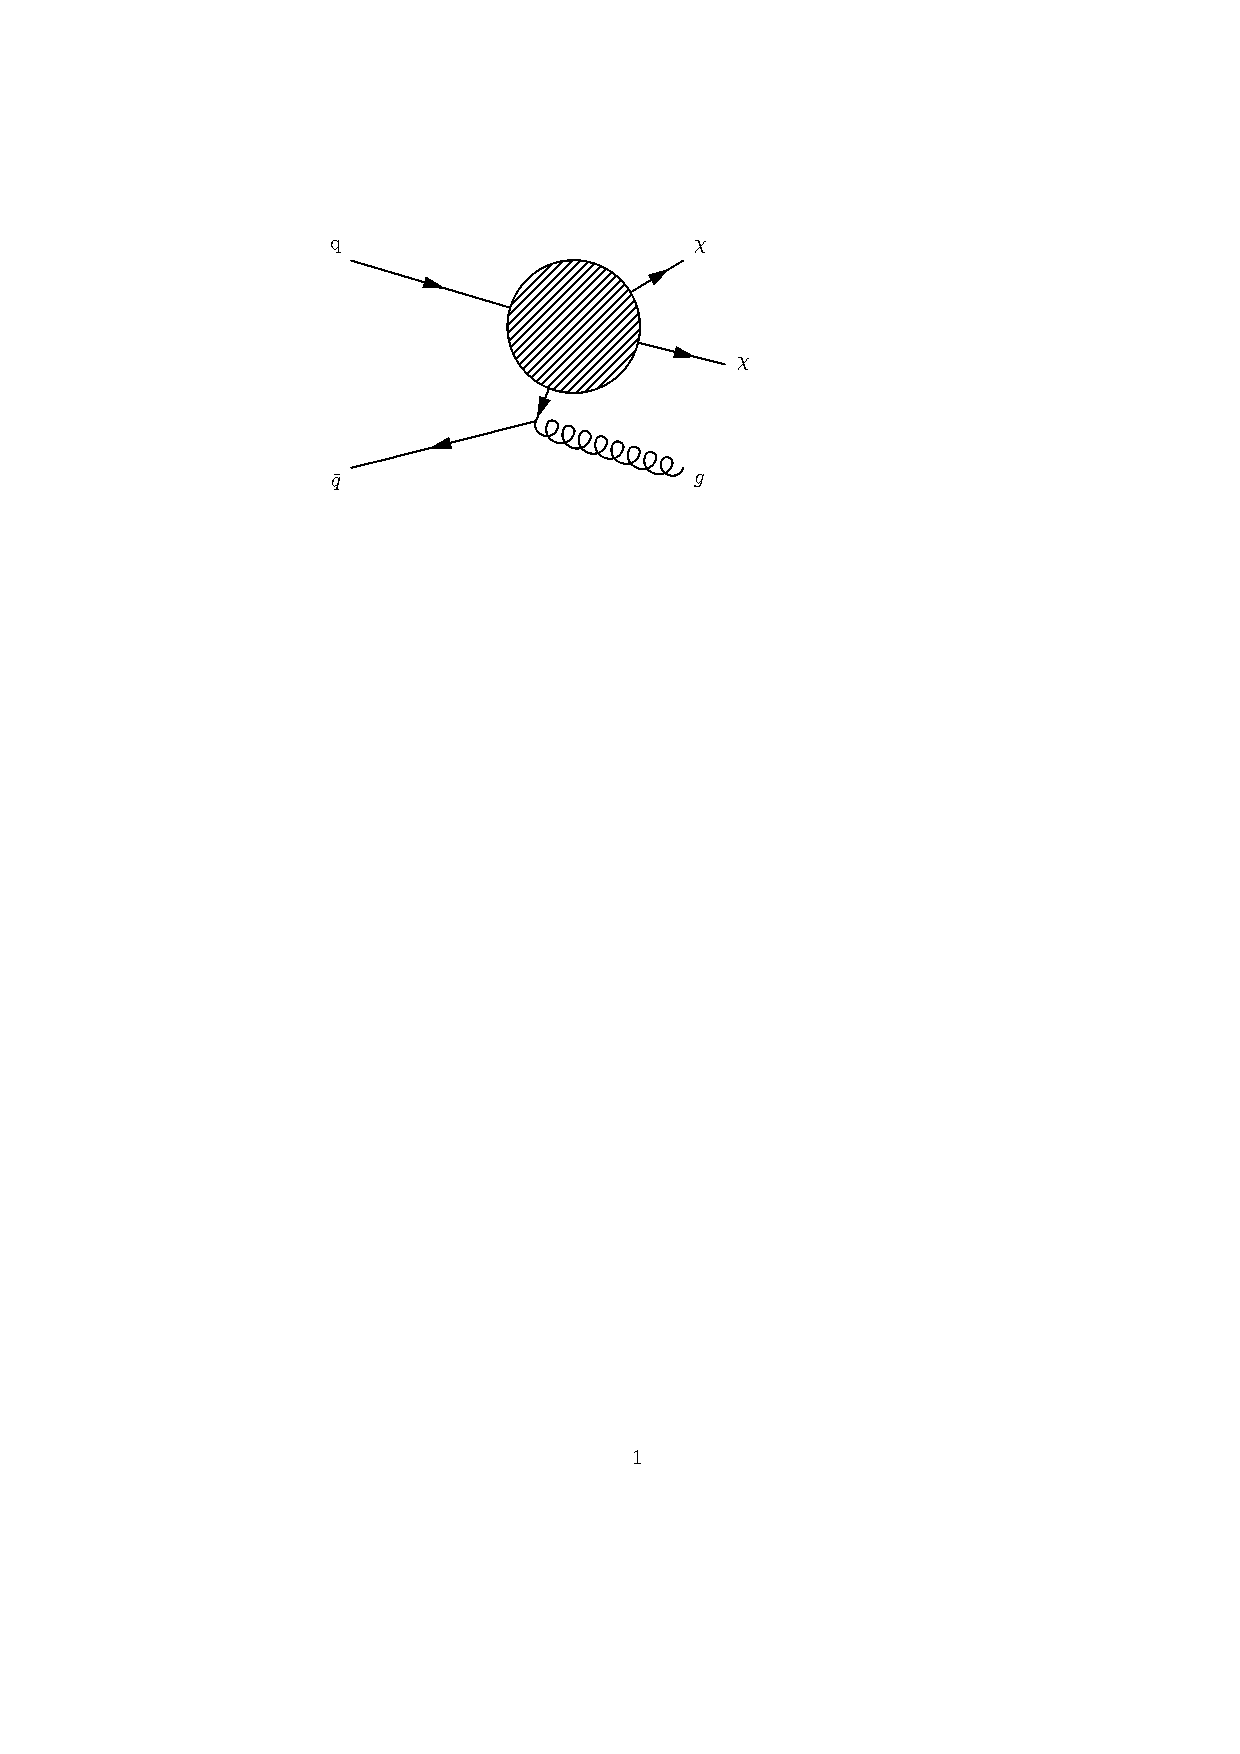
\includegraphics[trim=5cm 21cm 8cm 3.9cm, clip=true, width=0.5\textwidth]{effectiveD.pdf}
    }
    \hfill
    \subfloat[Feynman diagram describing the vector mediator model. \label{fig:opfeyn:b}]{%
      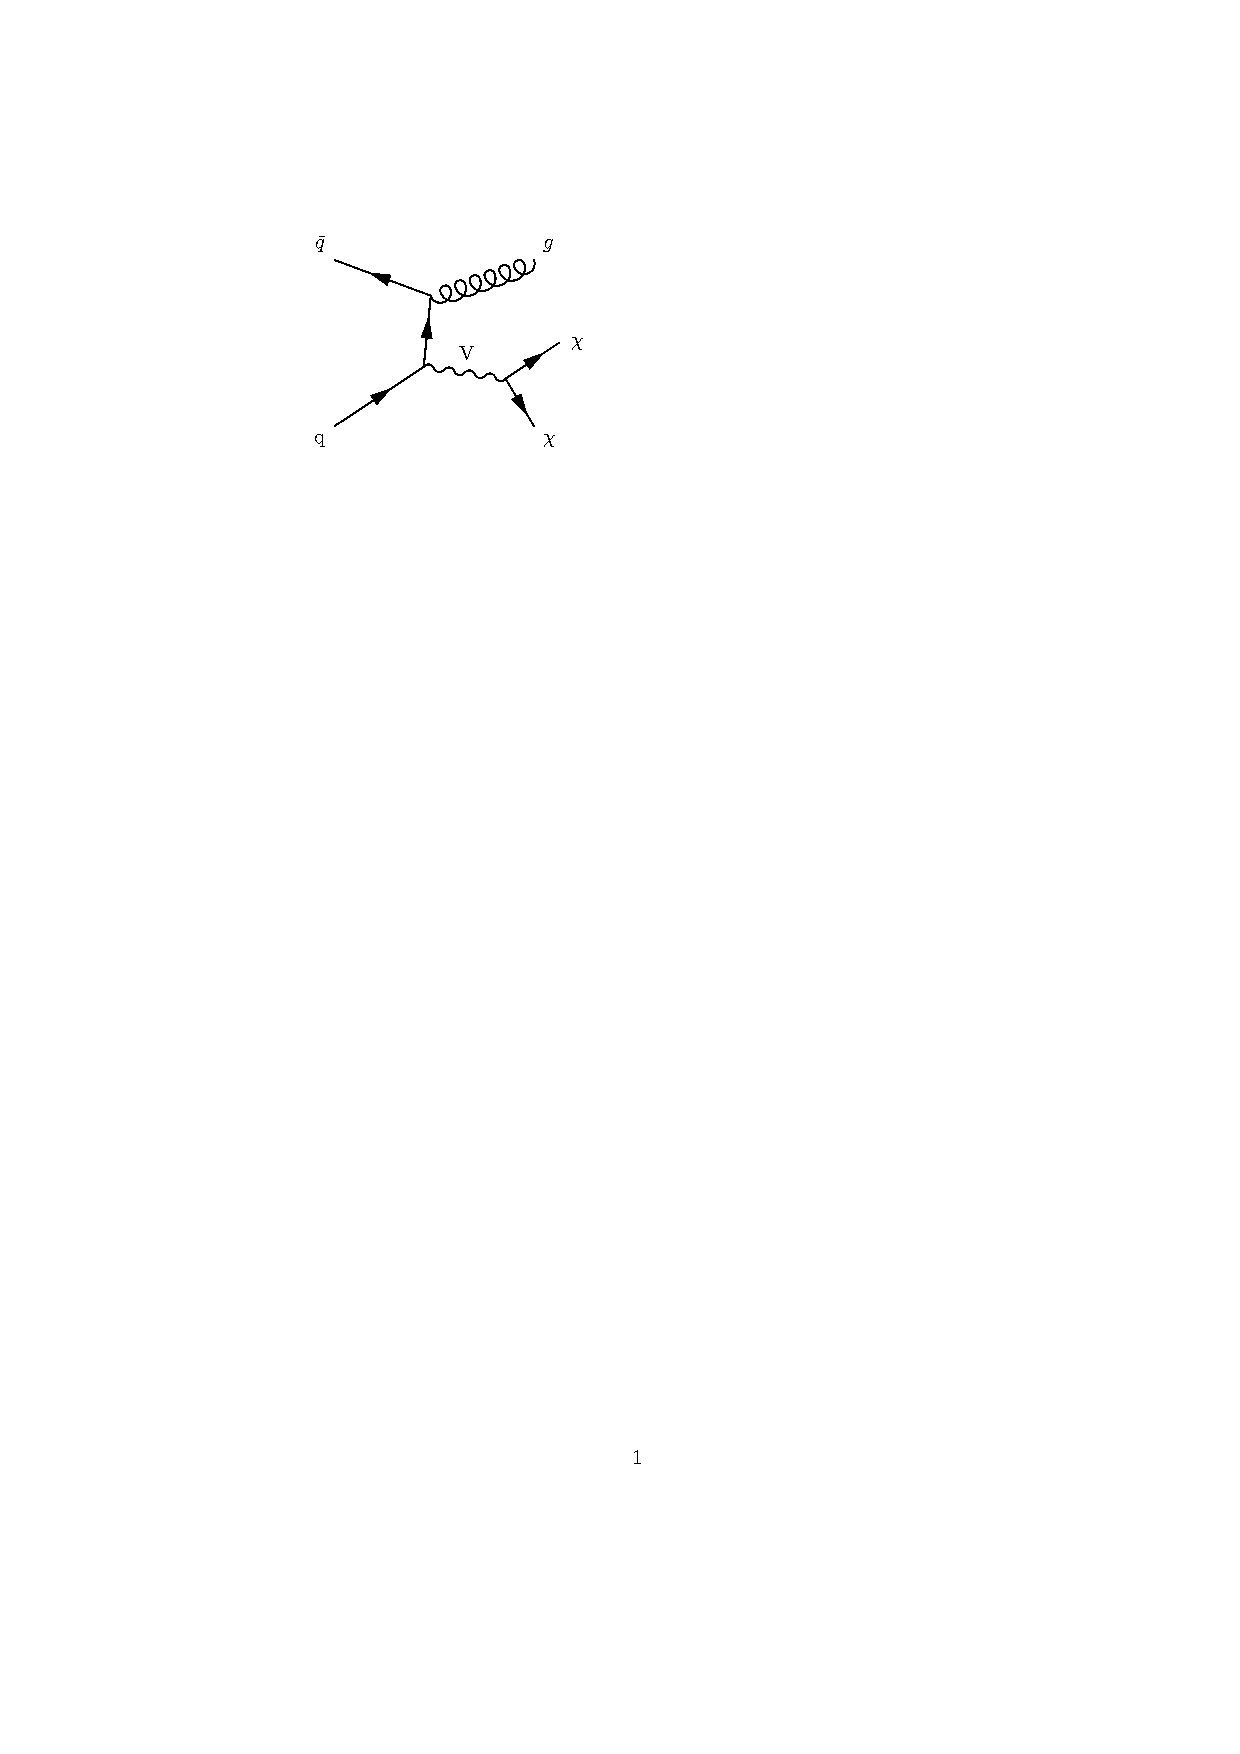
\includegraphics[trim=5cm 22cm 10cm 3.9cm, clip=true, width=0.5\textwidth]{vectorboson.pdf}
    }
    \caption{Feynman diagrams describing the used signal models.}
    \label{fig:opfeyn}
  \end{figure}
Another model which is considered is when the \abbrWIMP mass is close to the mediator mass. Then the effective theory fails and the process is assumed to be described by \figureref{fig:opfeyn:b}. 

\subsection{Search for \abbrWIMPS}\label{sec:tb:subsec:WIMPS}
The search of \abbrWIMPS is based on a mono-jet analysis which is described in \subsectionref{sec:eo:subsec:mjet}. 

Since the search for \abbrWIMPS at the \abbrLHC is based on looking at so called $E_T^{Miss}$ it will be canonical since the experiment can no establish if a \abbrWIMP is stable on a cosmological time scale and thus if it is a dark matter candidate \citep{CERN-PH-EP-2012-210}. This means that if a candidate is found, it may still not be the dark matter that is needed to explain the cosmological observations.

The different theories discussed in \subsectionref{sec:tb:subsec:eft} requires some process in which quarks and anti-quarks are produced. This process happens in a lot of different accelerators. The main problem is that nothing has been found low energy levels. This is why it is very interesting that the \abbrLHC is undergoing a upgrade that will allow higher energy levels. With this the processes can be given higher energy and thus the produced particles can be comprised of higher mass. 

Through earlier experiments the mass of dark matter has been given a lower limit. \textbf{WHAT?!?!}

What is it? Why at \abbrCERN/\abbrATLAS? Candidates?

\abbrWIMPS, wimps as candidates.
How is this detectable at \abbrATLAS? Finish with this. Refer next chapter and that neutralinos are a candidate. \textbf{(THEY ARE MAJORANA PARTICLES! so does not coincide with our effective field theory.)}

\newpage
\section{Experimental overview}\label{sec:experiment}
What was used in this research and what needs to be explained?
\subsection{\abbrLHC}
The Large hadron collider (\abbrLHC) is a particle accelerator located at \abbrCERN near Geneva in Switzerland, see \figureref{fig:lhc}. The accelerator was built to explore physics beyond the standard model and to make more accurate measurements of standard model physics. Before it was shut down for an upgrade in 2012 it was able to accelerate two proton beams to such a velocity that they had an energy of 4 TeV which gives a center of mass energy, $\sqrt{s}=8$ TeV. It should be noted that the proton beam is not homogeneous, it is comprised of bunches of protons with enough spacing that bunch collisions can happen independent of each other.Apart from the energy, the ability for an accelerator to produce interactions can be calculated through the instantaneous luminosity of the \abbrLHC was $10^{34}$ cm$^{-2}$s$^{-1}$ or $10$nb$^{-1}$s$^{-1}$ where 1 barn(b)$=10^{-24}$ cm$^2$. All values taken from \citep{lumires}.
\begin{figure}[H]
\begin{center}
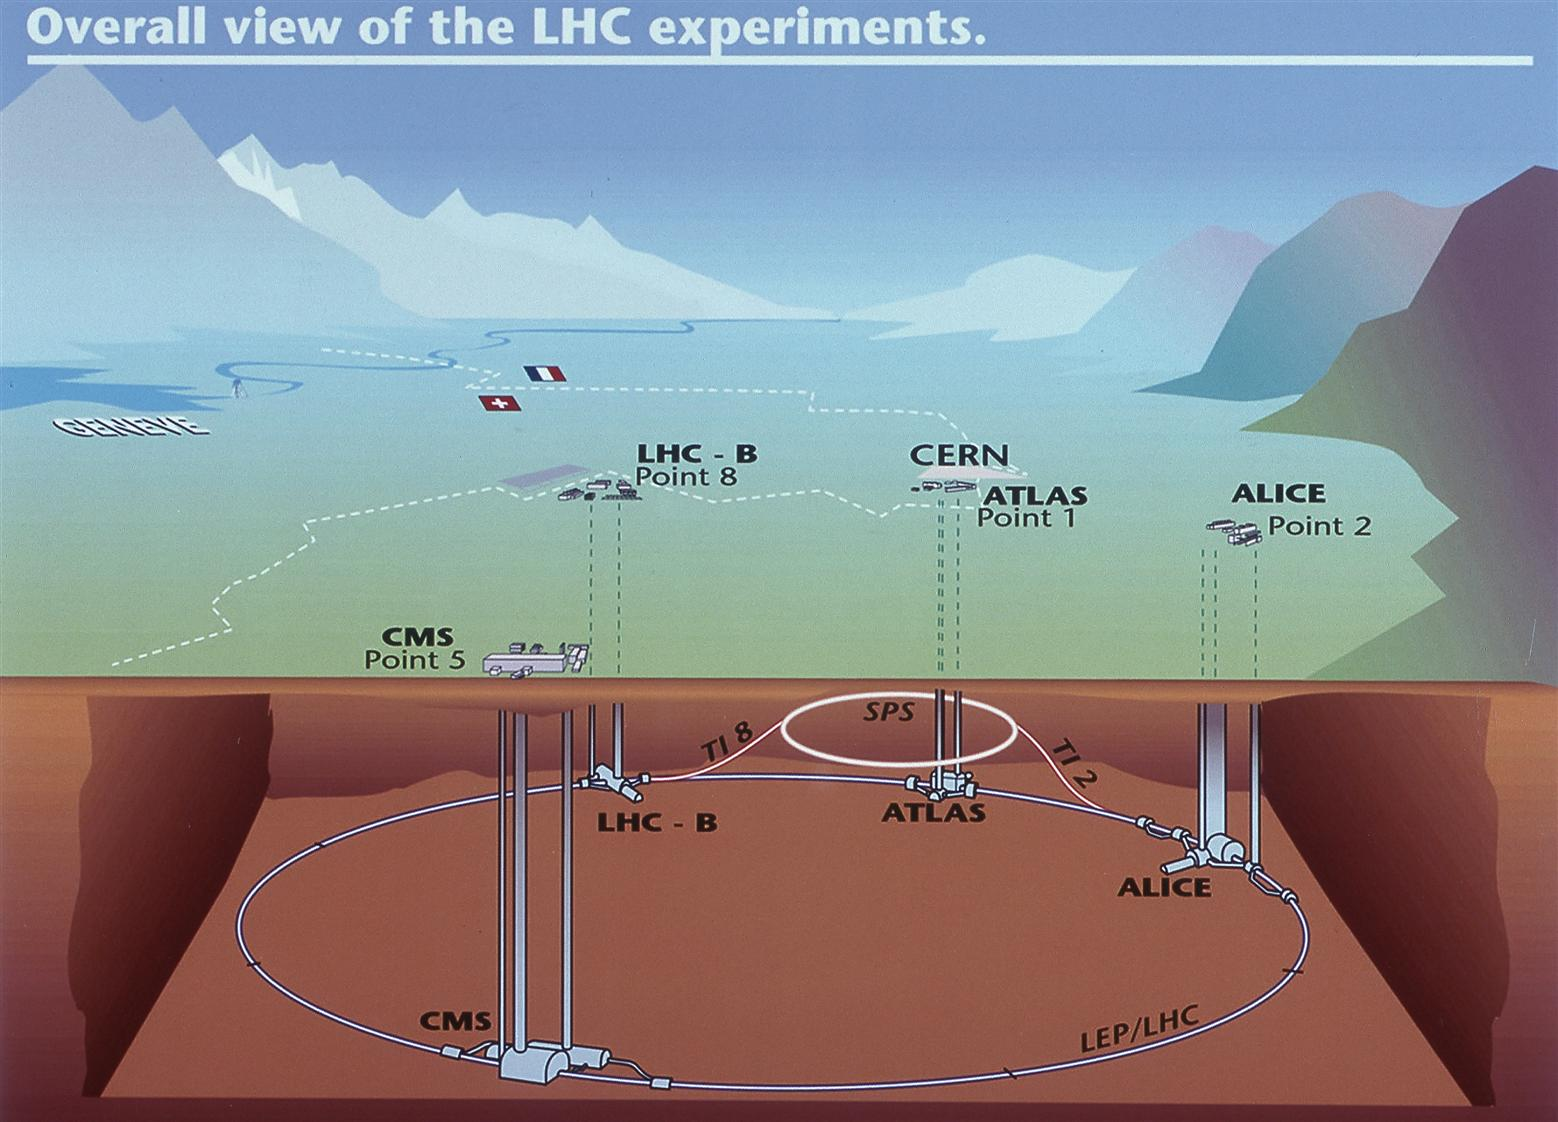
\includegraphics[width=\linewidth]{lhc.jpeg}
\caption{Figure showing the \abbrLHC and the different detector sites\citep{lhcimage}}
\label{fig:lhc}
\end{center}
\end{figure}
The instantaneous luminosity can be defined in different ways depending on how the collision takes place. For two collinear intersecting particle beams it is defined as:
\begin{equation}
\mathscr{L} = \frac{fkN_1 N_2}{4\pi \sigma_x \sigma_y}
\end{equation}
where $N_i$ are the number of particles in each of the bunches, f is the frequency at which the bunches collide , k the number of colliding bunches in each beam, and $\sigma_x$ ($\sigma_y$) is the horizontal (vertical) beam size at the interaction point. Since the instantaneous luminosity increases quadratically with more particles in each bunch this would be a good strategy. However aside from the difficulties to create and maintain a beam with more particles, a large $N_i$ increases the probability for multiple collisions per bunch crossing, referred to as pile-up. Pile up will be a key aspect which is described more in \subsectionref{sec:eo:subsec:pile}. 

The expected number of events can be calculated by using the instantaneous luminosity through the following:
\begin{equation}
N=\sigma \int \mathscr{L} dt := \sigma \Lagr
\end{equation}
where $\Lagr$ is the luminosity and $\sigma$ is the cross section which is often measured in barn.
The luminosity is a measurement of total number of interactions that have occurred over time. Before the \abbrLHC was shut down this values was 20.8 fb$^{-1}$.

The cross section is defined through the integral of the differential cross section, as explained in \subsectionref{sec:tb:subsec:qm}, over the whole solid angle:
\begin{equation}
\sigma = \oint d\Omega \frac{d\sigma}{d\Omega}
\end{equation}
The cross section is therefore a measure of the effective surface area seen by the impinging particles, and as such is expressed in units of area. The cross section is proportional to the probability that an interaction will occur. It also provides a measure of the strength of the interaction between the scattered particle and the scattering center.
Further details can be found in reference~\citep{Herr:2006}

\subsection{\abbrATLAS}
As seen in \figureref{fig:lhc}, there are several detectors at \abbrCERN. One of these is a large toroidal \abbrLHC apparatus (\abbrATLAS) which is a general purpose detector that uses a toroid magnet. Its goal is to observe several different production and decay channels. The detector is composed of three concentric sub-detectors, the Inner detector, the Calorimeters and the Muon spectrometer \citep{1129811}.

The Inner detectors main job is to detect the tracks of the particles and their interaction with the material in the detector.

The Calorimeters, the electromagnetic and hadronic, are used to calculate the energy contained in the different particles (electromagnetic get this and that, hadronic get this and that). 

The Muon spectrometer is used to detect signs of muons, which will simply pass through the other detectors without leaving a trace.

From this, it is known that neutrinos, and as assumed in this thesis \abbrWIMPS pass through all the detectors without leaving a trace.
\subsection{Coordinate system}
The coordinate system of ATLAS, seen in \figureref{fig:coordinatesystem} is a right-handed coordinate system with the x-axis pointing towards the centre of the LHC tunnel, and the z-axis along the tunnel/beam (counter clockwise) seen from above. The y-axis points upward.
The origin is define as the interaction point.
A cylindrical coordinate system is also used for the transversal plane. (R,$\phi$,Z).
For simplicity the pseudorapidity of particles from the primary vertex is defined as:
\begin{equation}
\eta = - \ln( \tan\frac{\theta}{2})
\end{equation}
where $\theta$ is the polar angle (xz-plane) of the particle direction measured from the positive z-axis. 
$\eta$ is through this definition invariant under boosts in the z-direction.

It is quite common to calculate the distance between particles and jets in the $(\eta,\phi$) plane, $d=\sqrt{\Delta \eta + \Delta \phi}$  

\begin{figure}[ht]
\begin{center}
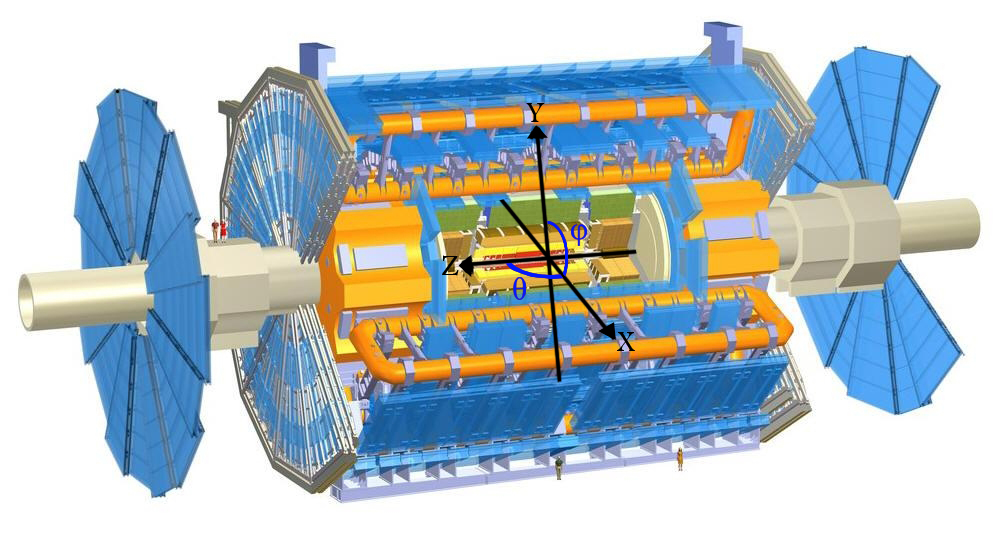
\includegraphics[width=\linewidth]{particle_collider.jpg}
\caption{Figure showing the \abbrATLAS detector and the definition of the orthogonal Cartesian coordinate system. Image altered from\citep{coordimage}}
\label{fig:coordinatesystem}
\end{center}
\end{figure}

\subsection{Reconstructing data}
To be able to compare the emulated data to measurable data it is important to include effects of the detectors. This is done using so called smearing functions which try to emulate the reconstruction of data. 

The reconstruction process of data \citep{1129811}, is based on what response is given from the detectors. It is affected by pile-up and the energy of that which is detected. 
The reconstruction process is not specifically used in the thesis, however the smearing functions are discussed in \sectionref{sec:vali:subsec:smear}.

\subsection{Pile-up}\label{sec:eo:subsec:pile}

Pile-up is defined as the average number of proton-proton collisions that occur per bunch crossing per second. It is denoted as $\obs{\mu}$. $\mu$ can be calculated by adjusting a Poisson distribution to fit the curve created by the number of interactions per bunch crossing at a given luminosity. When this is done $\mu$ will be the mean value of the Poisson distribution.


\subsection{Mono-jet analysis}\label{sec:eo:subsec:mjet}

\begin{figure}[ht]
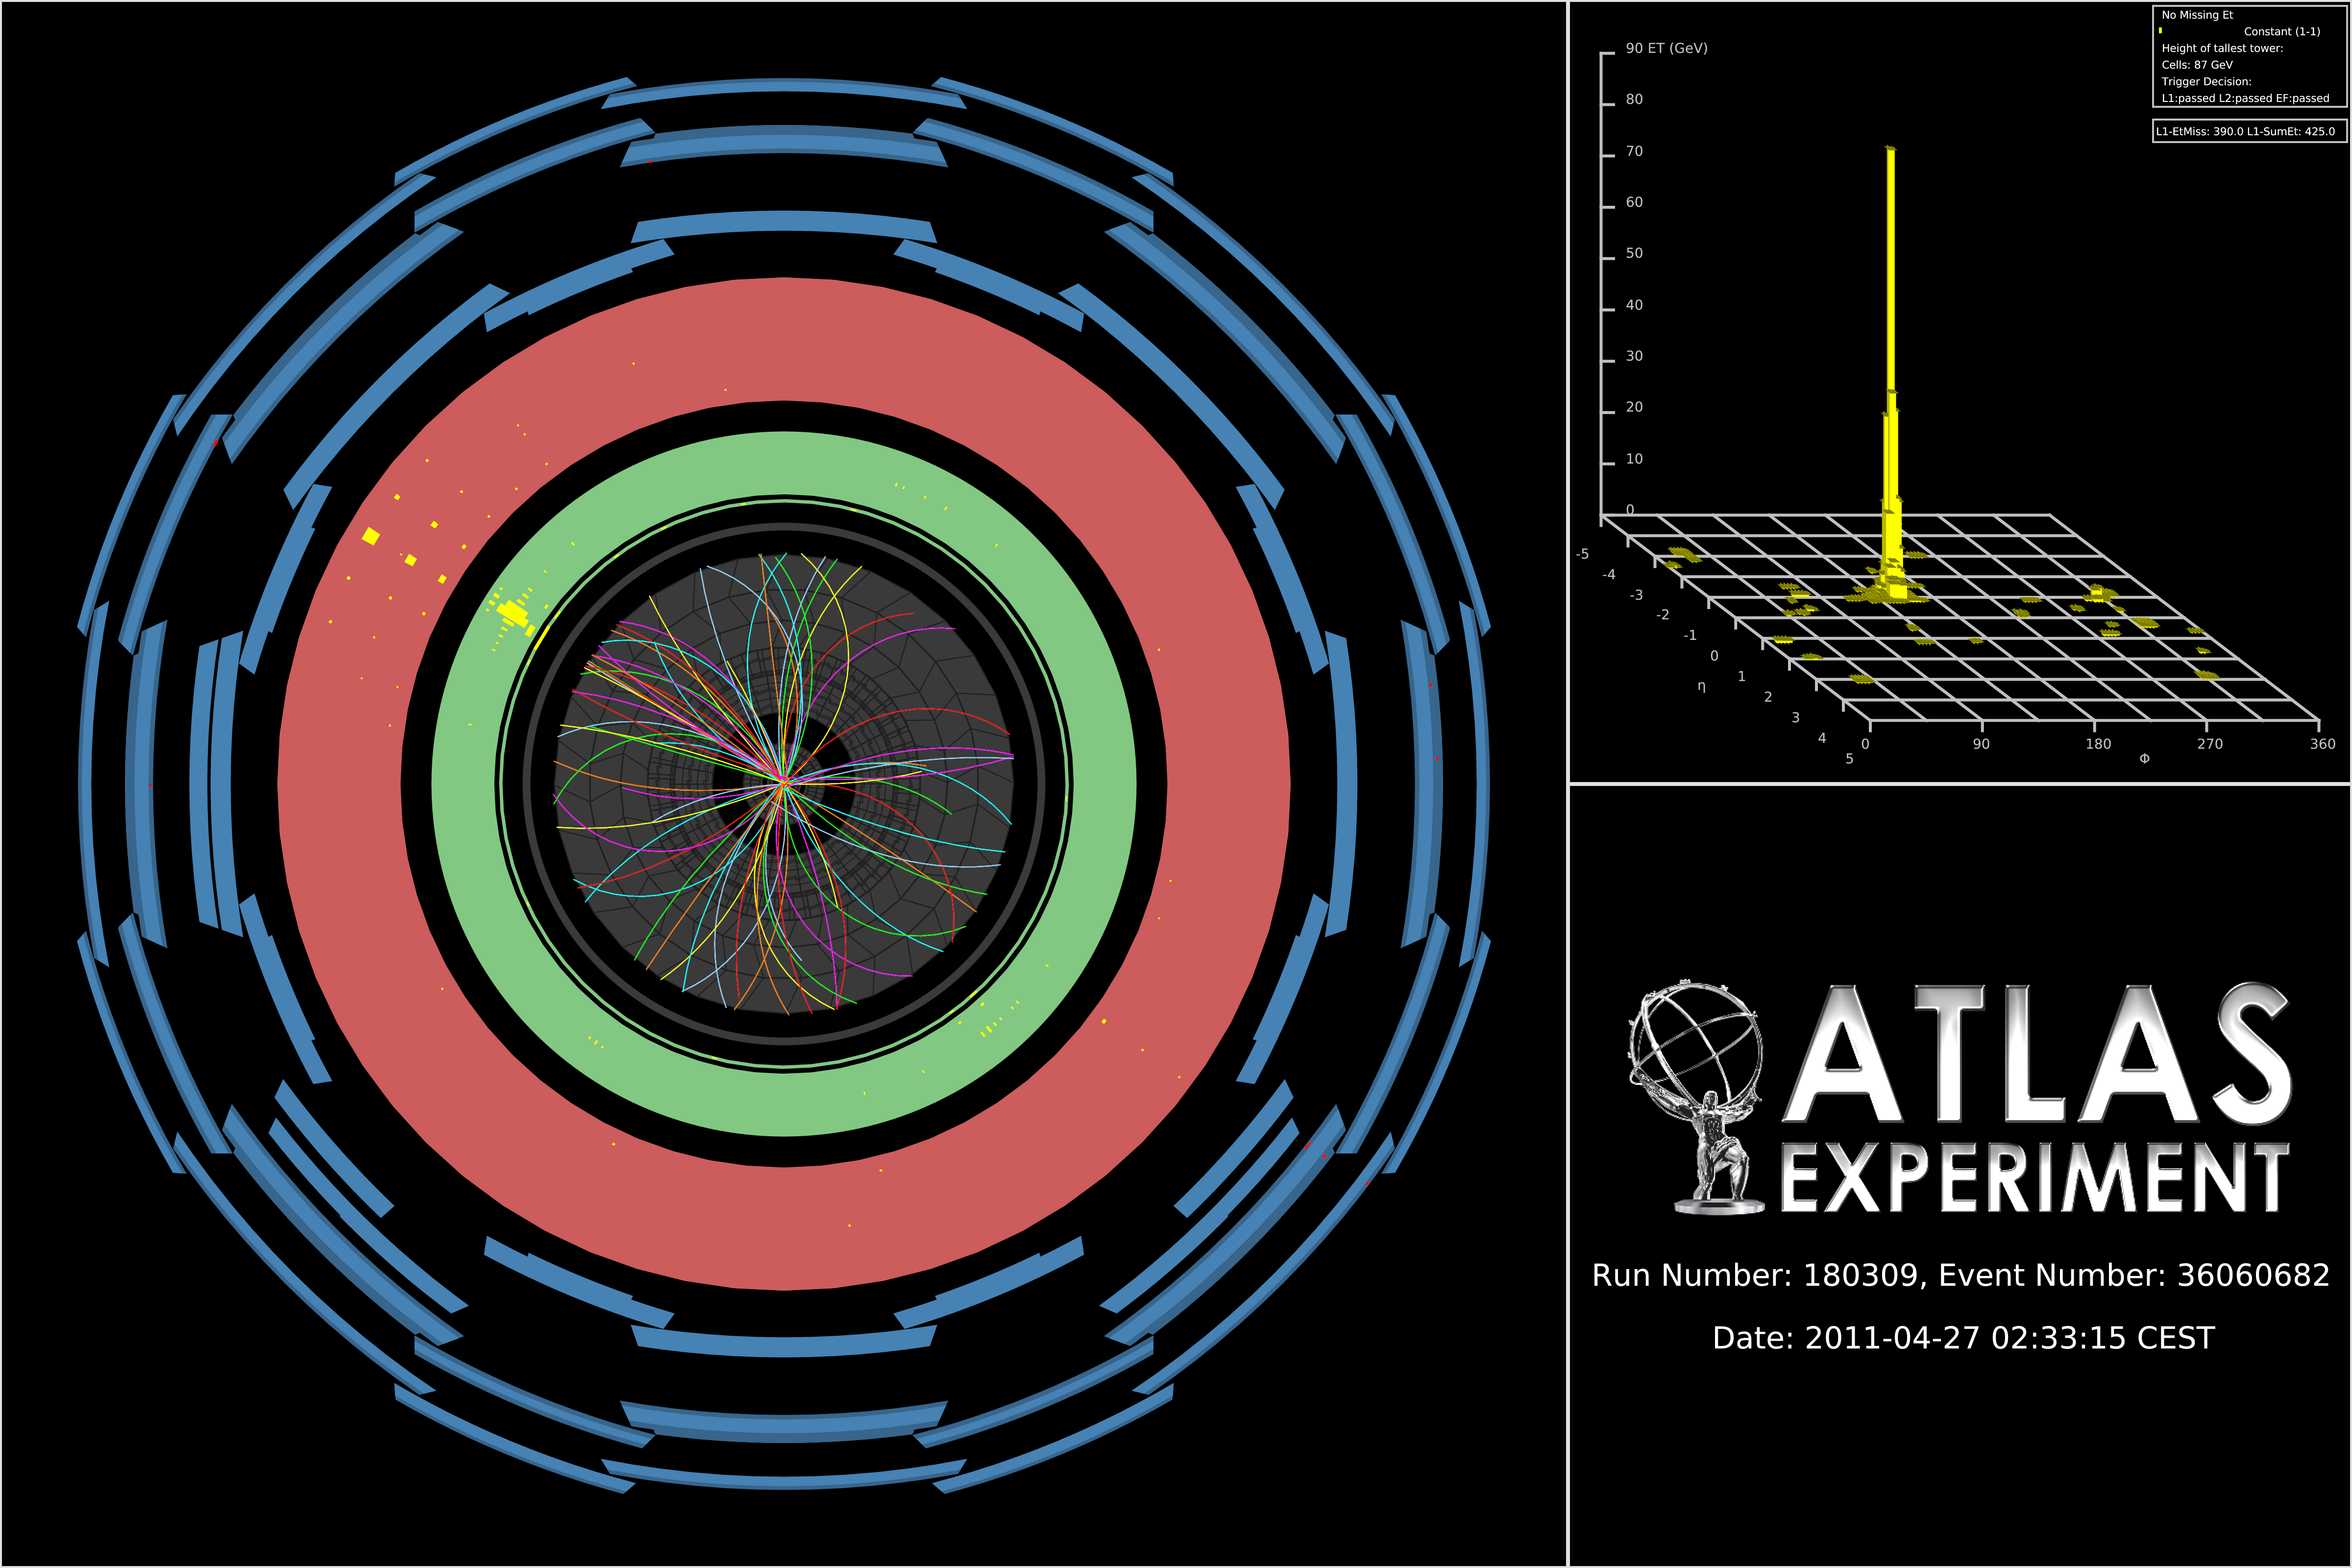
\includegraphics[width=\linewidth]{monojetbig.png}
\caption{Image of a mono-jet event \citep{monojet}.}
\label{fig:monojet}
\end{figure}

Transversal energy since it is known that it is almost zero before the collision and that it is unknown the amount of energy before and after in the z-direction. (Hard to create a detector that does not block the beam.)

When measuring the transversal energy one can in some interactions find inconsistencies, such as jets that are in excess in one direction. In \figureref{fig:monojet} one can see a high energetic jet which gives an excess of transversal energy in one direction after the collision. Since there is no balancing jet there must be transversal energy that is not detected, denoted $E_T^{Miss}$, since it was close to zero before the collision. This gives an indication that there energy to balance this that simply can not be detected. This could for instance be neutrinos or the sign of a new particle.

Jets are showers of particles that are produced at collisions. They are composed of highly energetic quarks and/or gluons. Since the gluons have self interaction, they s split into even more gluons which then results in shower of particles moving in the same direction. In the final stages the quarks and gluons can combine to form larger particles. It is by measuring these end products that one can gain more information about the collision which created the jet.

There are two main concepts to the analysis, signal and background. The signal is what theoretically should be detected by a assumed process. In this thesis the different dark matter processes, from \subsectionref{sec:tb:subsec:eft}, will constitute different signals. However to know that the missing energy is sign of the signal then one must understand all the other components that could contribute to the missing energy.

The background comprises of all the background processes that occur and that could contribute to the missing energy. By finding so called Control regions, where background process are in excess, one can model the missing energy by how many neutrinos come from the processes. 

\subsection{Phase II high luminosity upgrade}\label{sec:eo:subsec:hlu}
Talk about the upgrade schedule. \citep{ATLAS:LOI2}

The key question is how the signals are affected by the increase of luminosity and pile-up.

I am looking at the upgrade which will be done at \abbrCERN and will be completed around 2022-2023 and is denoted High Luminosity-\abbrLHC Phase 2 upgrade. When this is running the following is expected:
\renewcommand{\arraystretch}{1.5} %Change height of tabel
\begin{table}[H]
\begin{center}
    \begin{tabular}{ | l | l | l |}
    \hline
    Entity & Expected & Last run (2012) \\ \hline
  	Luminosity & 1000-3000 fb$^{-1}$ & 20.8 fb$^{-1}$ \\ \hline
  	Pile-up & $\obs{\mu}=200$ & $\obs{\mu}=20.7$ \\ \hline
  	Center of mass energy & $\sqrt{s}=14$ TeV &  $\sqrt{s}=8$ TeV \\ \hline
  	\end{tabular}
  	
  	\caption{Expected running values for the Phase II HL-upgraded \abbrLHC with older values for comparison. REFERENCE?}
  	\label{tab:expectvalues}
  	\end{center}
    \end{table}
    \renewcommand{\arraystretch}{1.0}  %Back to default
Taken from "a short explanation of different terminology by me" Find a cern source.
Assumed effects, timespan when will it be done?

\subsection{Monte Carlo simulation}
As mentioned before, in this thesis only emulated data has been used. To do this a program called MadGraph.

MadGraph \citep{madgraph} starts with Feynman diagrams and then generates simulated events based on lots of different parameters. To create correct simulations for this analysis PYTHIA has been used.

PYTHIA \citep{Sjostrand:2008} is a package which adds the correct description of jets and missing energy to MadGraph.

These programs are based on a Monte Carlo simulation.

"Monte Carlo (MC) simulated event samples are used to develop and validate the analy-
sis procedure and to evaluate the subdominant SM backgrounds as well as the expected
signal yields. The effect of multiple proton-proton collisions from the same or different bunch crossings is incorporated into the simulation by overlaying mini-mum bias events generated using PYTHIA onto hard scatter events. Simulated events are weighted to match the distribution of the number of interactions per bunch crossing observed in data."

\subsection{ROOT}
ROOT is a tool used for programming high energy physics related tools \citep{root}.

